\documentclass[a4paper,12pt]{article}
\usepackage{graphicx}
\usepackage{subcaption}
\usepackage{lineno}
\usepackage{float}
\usepackage{amsmath}
\usepackage{bm}
 \usepackage[authoryear,round, longnamesfirst]{natbib}
\usepackage{textcomp}
\linenumbers
\linespread{1.6}
\begin{document}
\title{Title}
\author{Authors}
\maketitle

\section{Abstract}
\begin{enumerate}
\item There has been an increasing amount of papers that have been producing estimated activity centre distributions -the summed posterior distribution of estimated range centres from a Bayesian fit of a homogeneous Poisson model- and claiming them to be "species distribution models", when this is not the case. In this paper we will demonstrate that these activity centre distributions and predicted density surfaces are not the same.
\item We illustrate this point through simulation and modelling of real data using the \textbf{secr} package \citep*{Efford}. We simulate using a grey scale image of the Mona Lisa, using the intensity of greyscale as the density of the "population". Then simulating from three different arrays on this surface, produce estimated activity centre surfaces and compare to the true density image, using models assuming constant density and models with covariates. We also use camera-trap capture-recapture survey data of snow leopards in South Gobi, Mongolia.  We create predicted density surfaces as well as estimated activity centre distributions to draw comparisons between the two methods.
\item There were very apparent differences in the surfaces produced via simulation and using the snow leopard data. The activity centre distributions are not representative of the predicted density surface using \textbf{predictDsurface}. They are very array dependent, even in areas where arrays overlap there are very different surfaces produced. As you move further away from the centre of the array the density also decreases, reflecting the fall in the detection function as you move from the traps.
\item Overall the results produced by these activity centre distributions do not perform very well, the simulations demonstrate very apparent differences from the true density. With the snow leopard data, the results are surprising, producing some results that are not probable.
\end{enumerate}

\section{Introduction}
Spatial capture-recapture (SCR) models are a set of methods for modelling capture-recapture data obtained from detectors such as camera-traps, hair snag traps and live-capture surveys such that individuals can be identified. Using the location of the detectors (traps) and also the detections of individuals over several occasion (capture histories), a estimate of density of individuals within a population can be obtained as well as an estimate of population size \citep*{Borchers2012}.
In order to do this, a spatial model of the population and a spatial model of the detection process are fitted to the capture histories of detected individuals.  This can be done using inverse prediction and maximum likelihood as well as using data augmentation and Markov chain Monte Carlo methods.

SCR combines a state model describing the distribution of activity centres in the landscape and an observation model relating the probability of detecting an individual at a particular detector to the distance from a central point in each animal's home range.

Consider a survey in which $K$ traps are placed in a region containing animals having home ranges with fixed centres (also known as activity centres). Once an animal is caught in a trap it remains there until it is released. These traps are checked at regular intervals and marked in such a way that their complete capture history is known and are released.  There are $S$ trapping occasions, trap k is located at Cartesian co-ordinates $x_k$ and the location of traps within the survey are at $x=(x_1, ..., x_k)$. The number of unique animals caught are n. $\bm{X}$ is the animal's location and this is it's activity centre.

Let $\omega_{i}=1$ if animal $i$ was captured on any of the $s$ occasions and $0$ if otherwise. If animal $i$ was captured on trap $k$ on occasion $s$ ($s=1, ...,S$) then $\omega_{is}=1$ and $0$ otherwise. The capture history for animal $i$ is $\omega_{i}=(\omega_{i1}, ..., \omega_{iS})$. Let $p_{ks}(\bm{X};\bm{\theta})$ be the probability that an animal with activity centre at $x$ is caught in trap $k$ on occasion $s$, where $\bm{\theta}$ is the capture probability parameter vector. %Let $p_{.s}(\textbf{X};\bm{\theta})$ be the probability that it is caught in any one of the $K$ traps on occasion $s$ and $p_{.}(\textbf{X};\textbf{$\theta$})$ be the probability that it is caught at all over the $s$ capture occasions: $p_{.}(\textbf{X}_{i};\bm{\theta})=Pr(\omega_{i}=1| \textbf{X}_{i};\bm{\theta})$.

%\paragraph{We assume that the locations of animal activity centres $(\textbf{s}_1, ..., \textbf{s}_N)$ in a survey area, $A$, are generated by a Poisson process with Density ("intensity") $D(\textbf{s})$ at $\textbf{s} \in A$. The number of activity centres in $A$ (N) is a Poisson random variable: $N\sim Po(\mu_{N})$ where $\mu_{N}=\int_{A}D(\textbf{s})d\textbf{s}$. Hence the probability density function of activity centre locations,  given N is proportional to $D(\textbf{s})$ at s: $f(\textbf{s}_1, ..., \textbf{s}_N)=\prod_{i=1}^{N}f(\textbf{s}_{i})$, where $f(\textbf{s}_{i})=D(\textbf{s}_{i})/ \mu_{N}$. The number N and the locations, $\textbf{s}_1, ...,\textbf{ s}_N$, of activity centres follows a Poisson Point Process $f(\textbf{s}_1, ..., \textbf{s}_N)=e^{-\mu_{N}}\prod_{i=1}^{N}D(\textbf{s}_{i})=Po(\mu_{N})N!\prod_{i=1}^{N}f(\textbf{s}_{i})$. With N fixed, we have a Binomial Point Process: $\prod_{i=1}^{N}\frac{D(\textbf{s}_{i})}{\mu_{N}}=\prod_{i=1}^{N}f(\textbf{s}_{i})$. With N treated as random, we have a Poisson Point Process. Typically for Bayesian inference methods, a Binomial Point Process is usually assumed but a Poisson can also be used.} 

From \citep*{Borchers2008} the likelihood is the joint distribution of the n animals captured and their capture histories $\bm{\omega}_1, ..., \bm{\omega}_n$ is 
$$L(\bm{\phi},\bm{\theta} | n, \bm{\omega}_1, ..., \bm{\omega}_n) =  Pr(n | \bm{\phi}, \bm{\theta})Pr(\bm{\omega}_1, ..., \bm{\omega}_n | n, \bm{\theta}, \bm{\phi})$$ 
$\theta$ is the vector of capture function parameters and $\phi$ is a vector of parameters of the spatial point process governing animal density and distribution.

When activity centres occur according to a homogeneous Poisson process with rate parameter $D$, the likelihood is simplified to 
$$L(\bm{\theta},D) = \frac{{Da(\bm{\theta})}^{n}exp^{-Da(\bm{\theta})}}{n!} \times \binom{n}{n_1, ..., n_C}\prod_{i=1}^{n}\frac{\int Pr(\bm{\omega}_{i}|\textbf{X};\bm{\theta})d\textbf{X}}{a(\bm{\theta})}$$
 where 
$$Pr(\bm{\omega}_{i} | \bm{X};\bm{\theta}) = \prod_{s} \prod_{k} p_{ks}(\textbf{X};\bm{\theta})^{\delta_{k}(\bm{\omega}_{is})}{1-p_{.s}(\textbf{X}; \bm{\theta})}^{1-\delta_{.}(\bm{\omega}_{ks})}$$
and $a(\bm{\theta}) = \int p_{.}(\textbf{X}; \bm{\theta}) d\textbf{X}$. An estimate of density can be obtained from the MLE estimate of $\hat{\theta}$ and hence $\hat{a}(\hat{\bm{\theta}})$ from the conditional likelihood, D is then estimated from $\hat{D}=n/\hat{a}$. If the capture probability and $a$ depend on covariates such as $\bm{z}$ then $\hat{D}=\sum_{i=1}^{n}\hat{a}(\bm{z_i})^{-1}$.  D is a fn of covariates, log link it, and also can do splines

%Following from (Borchers and Efford, 2008) the probability of capture in any one of the $K$ traps is 

%\begin{eqnarray*}
%p_{.s}(\textbf{X}) & = & 1-exp\{-T_{s}\sum_{k=1}^{K}h(d_{k}(\textbf{X})\} \\
%& = & 1-e^{-T_{s}h_{.}(\textbf{X})}
%\end{eqnarray*}

%where $h_{.}(\textbf{X})$ is the the total hazard of capture given $X$, $h(d_{k}(\textbf{X}))$ is the capture hazard function for trap $k$ at distance $d_{k}(\textbf{X})$ from $X$.  It follow that the probability of being caught in trap $k$ on the occasion $s$ is $p_{ks}\{1-e^{h_{.}(\textbf{X})}\}(d_{k}(\textbf{X}))/h_{.}(\textbf{X}))$.

%The hazard model can take many forms that can be used for the capture function. see paper

By using the estimates of the density model parameters $\phi$ we can estimate the probability density function of animal home-range centres in area $A$: $\hat{\pi}=\hat{D}(\hat{X})/\int_{A} \hat{D}(\bm{X}) d\bm{X}$. Given individual $i$'s and it's capture history $\bm{\omega}_i$ and an estimate of the capture probability parameter vector $\bm{\theta}$, the probability density function of $\bm{X}$, the location of this individual's home range centre (activity centre). 
$$\hat{f}(\bm{X}_{i} | \bm{\omega}_{i}) = \widehat{Pr}(\bm{\omega}_{i} | \bm{X}_{i})\hat{\pi}(\bm{X}_{i})/\int_{A} \widehat{Pr}(\bm{\omega}_{i} | \bm{X})\hat{\pi}(\bm{X})d\bm{X}$$
And for a homogeneous Poisson process this simplifies to: $$\hat{f}(\bm{X}_{i} | \bm{\omega}_{i}) = \widehat{Pr}(\bm{\omega}_{i} | \bm{X}_{i})/ \int_{A} \widehat{Pr}(\bm{\omega}_{i} | \bm{X}))d\bm{X}$$

In several papers, there has been some confusion as to the difference between estimated activity centre distributions- the summed posterior distribution of estimated range centres from a Bayesian fit of a homogeneous Poisson model - and density surfaces \citep*{Dorazio2017, Kendall2016, Sollmann2011, Royle2009}. with the former even being referred to as a "species distribution model" \citep*{Dorazio2017} and states that this approach is useful even when the sources of spatial variation in population density are not known. In this paper we will illustrate that the two are not equivalent. There are various problems with interpreting these surfaces as "species distribution models" and "density surfaces", attention is only focused on individuals that were caught. The individuals that were not caught but were present are represented by a smoothly varying base level that dominates the outer regions of the plot. The surface also depends on sampling intensity, as more data is added the the surface will change shape systematically and the plots are prone to artefacts \citep*{Efford}.

\section{Materials and Methods}
\subsection{Simulation set up}

Estimated density surfaces and activity centre distributions are usually presented as image plots. This makes them easy for the reader to absorb and interpret. In order to present our argument and results in a way that is easy to interpret visually. We simulate data from a density surface model based on one of the most recognisable images in Western culture, the Mona Lisa. Using the Mona Lisa, we created a greyscale image from it, and used the intensity of the greyscale to be the density of the population. The lighter areas were areas of high density of activity centres. This density surface is shown in Fig. \ref{monalisaDpts}.

\begin{figure}[h!]
\centering
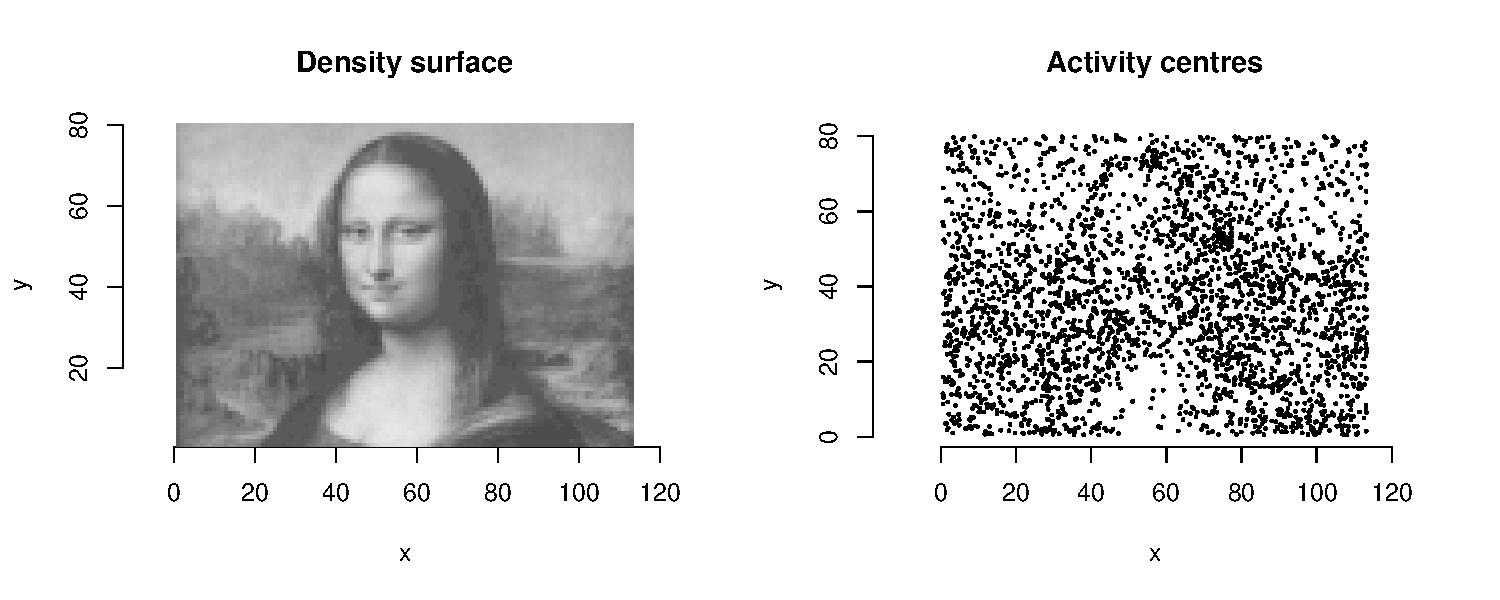
\includegraphics[width=1\textwidth]{monalisaDpts}
\caption{Density surface map map (left: dark is high density, light is low density) and the associated simulated population of 491 activity centres (right).}
\label{monalisaDpts}
\end{figure}

We conducted three simulated surveys of the population, using a 7x7 array of detectors with three different array centres (Fig. \ref{arrays}).

\begin{figure}[H]
\centering
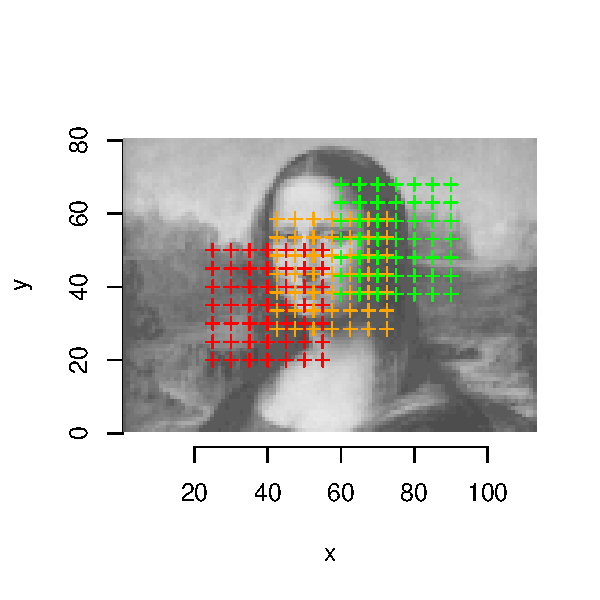
\includegraphics[width=0.5\textwidth]{arrays}
\caption{Detector arrays. Each array is a different colour.}
\label{arrays}
\end{figure}

For these simulated surveys, we used a half-normal detection function and set $g_0$, the probability of detection at a single detector placed in the centre of the home range to be 0.5 and $\sigma$, the spatial scale parameter to 2.5 \citep*{Efford2009}. The array was spaced such that it was of length 5m in the x-plane and 5m in the y-plane and so had an average spacing of 4m. Then we simulated a capture history for a single occasion on each array using the \textbf{sim.capthist} function.

\begin{figure}[H]
\centering
\includegraphics[width=0.4\textwidth]{detfn}
\caption{Detection function}
\label{detfn}
\end{figure}

Array 1 (red in Fig. \ref{arrays}) observed 53 animals with 82 detections in total, and 36 detectors being visited out of the 49 used (Fig. \ref{capthists}). Array 2 (yellow in Fig. \ref{arrays}) observed 56 animals with 89 detections overall and had 34 detectors that were visited (Fig. \ref{capthists}). Array 3 (green in Fig. \ref{arrays}) had 58 observed animals along with 102 detections, with 39 of the 49 detectors being visited (Fig. \ref{capthists}).

\begin{figure}[h]
\hbox{\hspace{-6em} \includegraphics[width=1.4\textwidth]{capthists}}
\caption{Captures across detectors on each array.}
\label{capthists}
\end{figure}

Additionally, we created a 10x10 array that covered most of the surface (Fig. 5a) and simulated another capture history for this. $g_0$ and $\sigma$ were kept the same as before in the previous simulations and the array was 8m in the x-plane and 6m in the y-plane with an average spacing of 6m between detectors. This array observed 125 animals with 168 detections in total and 77 detectors were visited out of 100 used (Fig. 5b).

\begin{figure}[h]
\centering
\begin{subfigure}[h]{0.4\textwidth}
\includegraphics[width=\textwidth]{"10x10 array"}
\caption{The 10x10 array.}
\label{10x10}
\end{subfigure}
\begin{subfigure}[h]{0.4\textwidth}
\includegraphics[width=\textwidth]{capthist}
\caption{Captures across detectors on the 10x10 array.}
\label{10x10 capt hist}
\end{subfigure}
\caption{Array and capture history}
\end{figure}

\subsection{Estimated activity centre surface from model with constant density}
After simulating these capture histories for these arrays, we then created an estimated activity centre surface for each of these simulations, using the fxi functions in the \textbf{secr} package. In this scenario we assumed a model with constant density and compared them to the true population density surface.

\subsection{Estimated activity centre surface from model with density depending on covariates}
The next step was to introduce covariates into our density model and see how this affected the contours. The covariates we initially introduced were the levels of red, green and blue from the original colour JPEG of the Mona Lisa, however the RGB levels were so highly correlated with the intensity of greyscale in the grey Mona Lisa that they were near perfect predictors of density and hence were not realistic to use in this scenario. Thus noise was added to these individual colour levels by adding random values from the Normal distribution with mean 1 and standard deviation of 0.1. Then we repeated the simulations for each of the arrays we created with a density model where density depended on the level of blue, red and green (with noise) individually, whilst $g_0$ and $\sigma$ were kept constant and a half-normal detection function again. For comparison, the predictDsurface function from secr was used to create an estimated density surface for comparison.

\subsection{Camera-trap survey of snow leopards in Tost, Mongolia}
To further investigate these estimated activity centre surfaces we use camera-trap survey data of snow leopards in the Tost Mountains of South Gobi. This is an important snow leopard habitat, characterized by rugged mountain ranges spread out with large stretches of steppe. Digital camera traps (Reconyx\texttrademark) using infrared and motion sensors to detect animal movement and low-glow monochrome illumination were used to sample snow leopard populations.  There were 41 cameras used, which depended on the minimum convex polygon of the sampled area that ranged from 920 to 1200 sq km.  A networking approach was used to place cameras in the field every 1-3km from another nearby camera. Precise camera trap locations were identified by surveying 2-5km on foot in the mountains, searching for sites where the chance of capturing a snow leopard was high. This was done by looking for sites with fresh snow leopard signs, such as scrapes or fresh urine markings. Most camera locations were characterized as saddles on ridgelines, overhanging rocks or steep canyon walls where snow leopards tend to mark and scrape. The best sites for installing camera traps were based on intuition and knowledge of snow leopard natural history from other sampling areas in the region. All cameras were left in the field for an average of 105.45 days. Snow leopards are known to use rugged mountains and tend to avoid flat terrain \citep*{Johansson2015}. From the camera traps, we obtained 99 snow leopard encounters from the sampling area, with 14 individuals detected. Any cubs following mothers were included in our analysis. Individuals were indentified following methods described by \citep*{Sharma2014}. Any snow leopards which could not be identified were discarded from the analysis. Each trap was characterized by the value of terrain ruggedness at its specific location, to within 90m. Additionally, we recorded topography of the trap location as saddle or canyon, and marked presence/absence of waterhole within 50m from the camera traps. We assumed no temporal effect on detection probability of snow leopards during the sampling period primarily because the study periods were restricted to a single season during each sampling session. Earlier analyses using conventional capture recapture methods did not indicate any temporal effects on capture probability. Therefore, we considered the entire sampling as a single occasion and session. In this analysis, we decided to fit a model where depended only on the value of terrain ruggedness at its specific location as this is the snow leopard's preferred habitat. $g_0$ and $\sigma$ were kept constant and used a hazard half-normal detection function. In this analysis, we again created predictions density surface contours usIng the\textbf{predictDsurface} function and an estimated activity centre surface using the \textbf{fx.total} function from the secr package.

\begin{figure}[H]
\centering
\includegraphics[width=0.5\textwidth]{tosttraps}
\caption{Placement of traps}
\label{tosttraps}
\end{figure}

\section{Results}
\subsection{Simulations with constant density model}

\begin{table}[H]
\centering
\begin{tabular}{rrrrr}
  \hline
 & beta & SE.beta & lcl & ucl \\ 
  \hline
D & 6.39 & 0.18 & 6.04 & 6.74 \\ 
  $g_0$ & -0.28 & 0.36 & -0.98 & 0.43 \\ 
  $\sigma$ & 1.10 & 0.09 & 0.91 & 1.29 \\ 
   \hline
\end{tabular}
\caption{Summary of model parameters for constant density model for array 1}
\end{table}

\begin{table}[H]
\centering
\begin{tabular}{rrrrr}
  \hline
 & beta & SE.beta & lcl & ucl \\ 
  \hline
D & 6.41 & 0.17 & 6.08 & 6.74 \\ 
  $g_0$ & 0.53 & 0.43 & -0.32 & 1.37 \\ 
  $\sigma$ & 0.92 & 0.09 & 0.75 & 1.09 \\ 
   \hline
\end{tabular}
\caption{Summary of model parameters for constant density model for array 2}
\end{table}

\begin{table}[H]
\centering
\begin{tabular}{rrrrr}
  \hline
 & beta & SE.beta & lcl & ucl \\ 
  \hline
D & 6.32 & 0.16 & 6.01 & 6.62 \\ 
  $g_0$ & -0.21 & 0.30 & -0.80 & 0.38 \\ 
  $\sigma$ & 1.20 & 0.08 & 1.04 & 1.37 \\ 
   \hline
\end{tabular}
\caption{Summary of model parameters for constant density model for array 3}
\end{table}

From the constant density model, our estimates of abundance were 537 (SE=93.9), 550 (SE=89.8) and 501 (SE=75.6) respectively. Confidence intervals for abundance were (385, 758), (403, 760) and (375, 675) for each individual array.

\begin{figure}[H]
\centering
\hbox{\hspace{-3em} 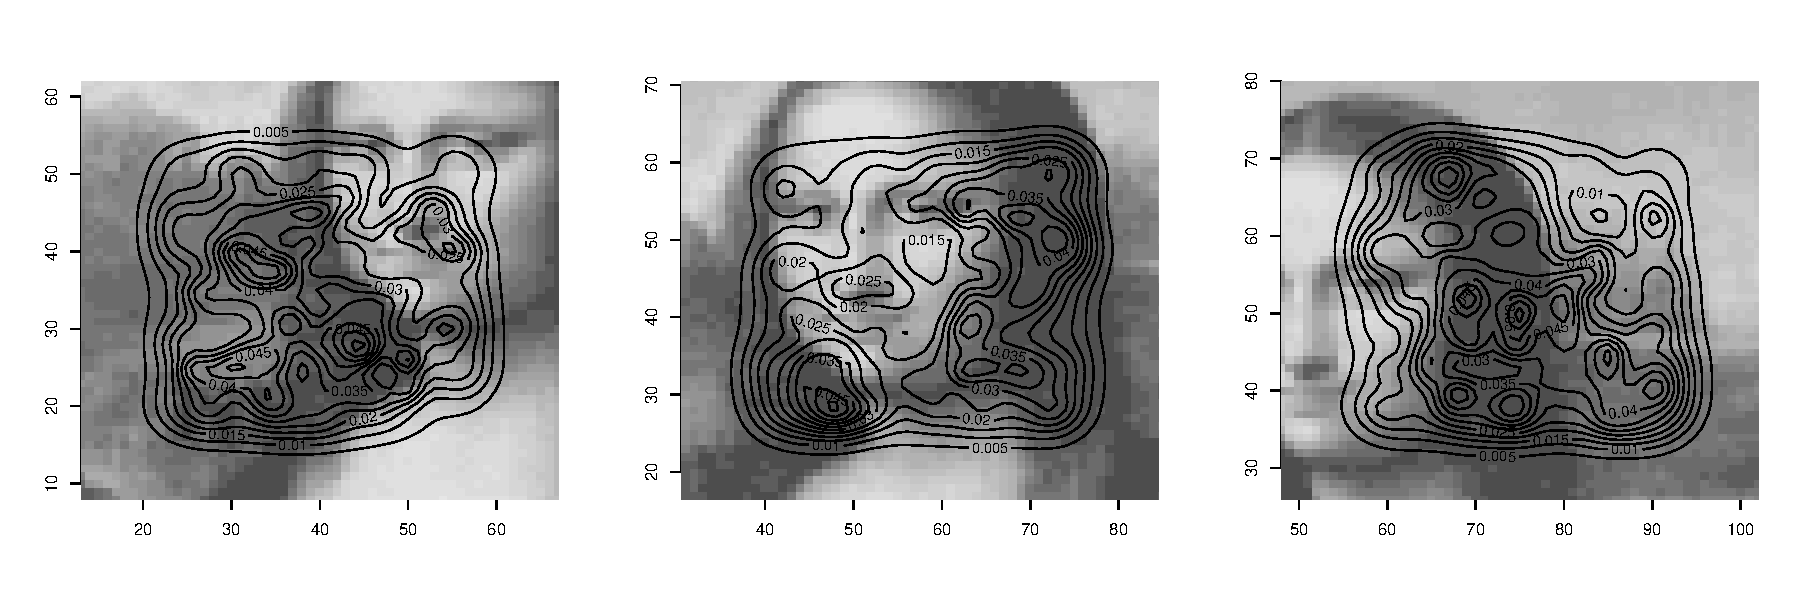
\includegraphics[width=1.2\textwidth]{localests}}
\caption{Local estimates of activity centre densities}
\label{localests}
\end{figure}

\begin{figure}[H]
\centering
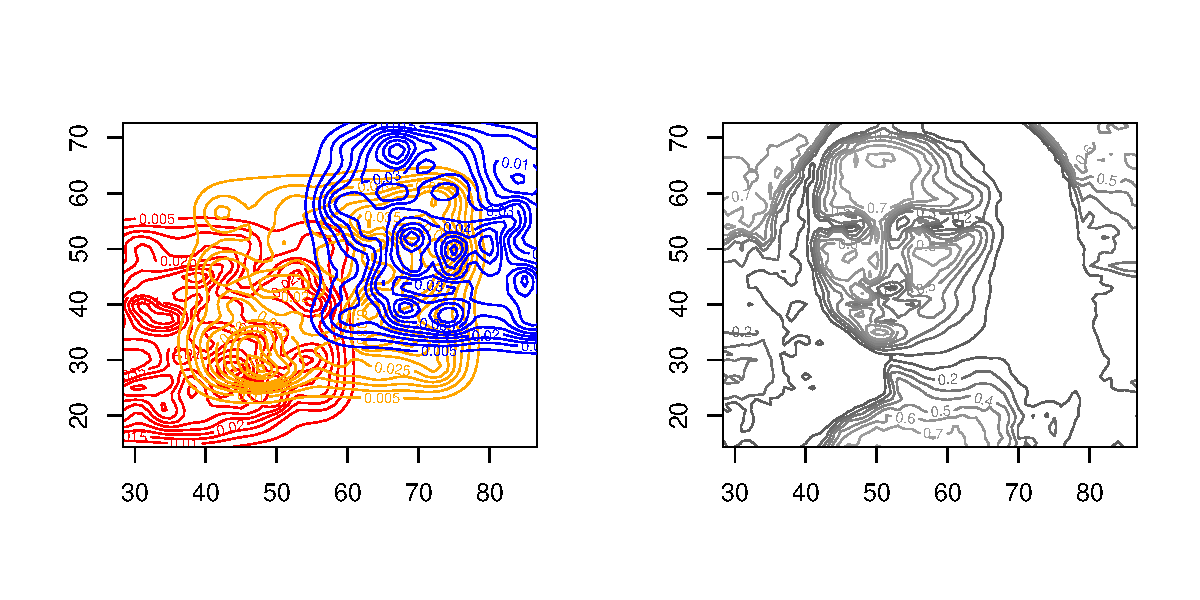
\includegraphics[width=\textwidth]{overlap}
\caption{Overlap of activity centre density contours}
\label{overlap}
\end{figure}

For the 10x10 array we obtained an abundance estimate of 506 animals, a standard error of 68.9 and a 95\% confidence of (393,667).

\begin{table}[ht]
\centering
\begin{tabular}{rrrrr}
  \hline
 & beta & SE.beta & lcl & ucl \\ 
  \hline
D & 6.33 & 0.14 & 6.05 & 6.61 \\ 
  g0 & 0.27 & 0.32 & -0.36 & 0.90 \\ 
  sigma & 0.97 & 0.07 & 0.84 & 1.11 \\ 
   \hline
\end{tabular}
\caption{Summary of model parameters for 10x10 array constant density model}
\end{table}

\begin{figure}[h]
\centering
\includegraphics[width=\textwidth]{10x10}
\caption{True density contour (left) compared with activity centre contours from the 10x10 array}
\label{10x10}
\end{figure}


\subsection{Simulations with density model including covariates}

%blue

\begin{table}[H]
\centering
\begin{tabular}{rrrrr}
  \hline
 & beta & SE.beta & lcl & ucl \\ 
  \hline
D & 6.93 & 0.38 & 6.19 & 7.67 \\ 
  D.B.N & -3.53 & 2.58 & -8.60 & 1.53 \\ 
  $g_0$ & -0.26 & 0.36 & -0.97 & 0.44 \\ 
  $\sigma$ & 1.10 & 0.09 & 0.92 & 1.29 \\ 
   \hline
\end{tabular}
\caption{Summary of model parameters for blue covariate model for array 1}
\end{table}

\begin{table}[H]
\centering
\begin{tabular}{rrrrr}
  \hline
 & beta & SE.beta & lcl & ucl \\ 
  \hline
D & 7.40 & 0.33 & 6.75 & 8.05 \\ 
  D.B.N & -9.93 & 4.93 & -19.60 & -0.26 \\ 
  g0 & 0.45 & 0.43 & -0.39 & 1.29 \\ 
  sigma & 0.92 & 0.09 & 0.75 & 1.10 \\ 
   \hline
\end{tabular}
\caption{Summary of model parameters for blue covariate model for array 2}
\end{table}

\begin{table}[H]
\centering
\begin{tabular}{rrrrr}
  \hline
 & beta & SE.beta & lcl & ucl \\ 
  \hline
D & 6.39 & 0.29 & 5.82 & 6.96 \\ 
  D.B.N & -0.38 & 1.36 & -3.06 & 2.29 \\ 
  g0 & -0.21 & 0.30 & -0.80 & 0.38 \\ 
  sigma & 1.20 & 0.08 & 1.04 & 1.37 \\ 
   \hline
\end{tabular}
\caption{Summary of model parameters for blue covariate model for array 3}
\end{table}

From the blue covariate model, we produced estimates of abundance of 489 (SE=86.6), 400 (SE=70.9), 495 (SE=77.0) on each array respectively alongside 95\% confidence intervals of (349, 694), (286, 569) and (368, 673).

\begin{figure}[H]
\centering
\includegraphics[width=\textwidth]{localestsblue}
\caption{Local estimates of activity centre contours using blue levels as a covariate on each array.}
\label{localestsblue}
\end{figure}

\begin{figure}[H]
\centering
\includegraphics[width=\textwidth]{densitypredsblue}
\caption{Density contours using predictDsurface for blue covariate on each array.}
\label{densitypredblue}
\end{figure}

For the 10x10 array, an abundance estimate of 486 was obtained with a standard error of 66.0 and a 95\% confidence interval of (378, 640).

\begin{table}[ht]
\centering
\begin{tabular}{rrrrr}
  \hline
 & beta & SE.beta & lcl & ucl \\ 
  \hline
D & 6.76 & 0.21 & 6.34 & 7.18 \\ 
  D.B.N & -2.45 & 1.05 & -4.52 & -0.39 \\ 
  g0 & 0.27 & 0.32 & -0.36 & 0.89 \\ 
  sigma & 0.98 & 0.07 & 0.84 & 1.11 \\ 
   \hline
\end{tabular}
\caption{Summary of model parameters for 10x10 array density model with blue covariate}
\end{table}

\begin{figure}[H]
\centering
\includegraphics[width=\textwidth]{10x10blue}
\caption{Density prediction (left), 10x10 activity centre contour using 10x10 array (centre) and 10x10 activity centre contour with constant density.}
\label{10x10blue}
\end{figure}

%red
%\begin{figure}[h]
%\centering
%\includegraphics[width=\textwidth]{localestsred}
%\caption{Local estimates of activity centres using red levels as a covariate on each array}
%\label{localestsred}
%\end{figure}

%\begin{figure}[h]
%\centering
%\includegraphics[width=\textwidth]{densitypredred}
%\caption{Density contours using predictDsurface for red covariate on each array.}
%\label{densitypredred}
%\end{figure}

%\begin{figure}[H]
%\centering
%\includegraphics[width=\textwidth]{10x10red}
%\caption{Density prediction (left), 10x10 activity centre contour using 10x10 array (centre) and 10x10 activity centre contour with constant density.}
%\label{10x10red}
%\end{figure}

%green
%\begin{figure}[H]
%\centering
%\includegraphics[width=\textwidth]{localestsgn}
%\caption{Local estimates of activity centres using green levels as a covariate on each array.}
%\label{localestsgn}
%\end{figure}
%\begin{figure}[H]
%\centering
%\includegraphics[width=\textwidth]{densitypredgreen}
%\caption{Density contours using predictDsurface for green covariate.}
%\label{densitypredgreen}
%\end{figure}
%\begin{figure}[H]
%\centering
%\includegraphics[width=\textwidth]{10x10g}
%\caption{Density prediction (left), 10x10 activity centre contour using 10x10 array (centre) and 10x10 activity centre contour with constant density.}
%\label{10x10g}
%\end{figure}

\subsection{Snow leopard data}

Our survey produced an abundance estimate of 15 snow leopards in the Tost Mountains with a standard error estimate of 1.347 and a confidence interval of (14.32, 20.78).

\begin{table}[ht]
\centering
\begin{tabular}{rrrrr}
  \hline
 & beta & SE.beta & lcl & ucl \\ 
  \hline
D & -9.55 & 0.29 & -10.12 & -8.98 \\ 
  D.stdGC & 0.22 & 0.34 & -0.44 & 0.89 \\ 
  $\lambda_0$ & -4.40 & 0.17 & -4.73 & -4.08 \\ 
  $\sigma$ & 8.85 & 0.08 & 8.69 & 9.01 \\ 
   \hline
\end{tabular}
\caption{Summary of fitted model for snow leopard data}
\end{table}

\begin{figure}[H]
\centering
\includegraphics[width=\textwidth]{density}
\caption{Comparison of predicted density surface (left) and activity centre distribution (right) for Tost}
\label{tostdensity}
\end{figure}

\begin{figure}[H]
\centering
\includegraphics[width=\textwidth]{logdensity}
\caption{Comparison of log predicted density surface (left) and activity centre distribution log density (right)}
\label{tostlogdensity}
\end{figure}

\begin{figure}[H]
\centering
\includegraphics[width=\textwidth]{stdGCvsd}
\caption{Comparison of stdGC covariate distribution map (left) and activity centre distribution (right)}
\label{stdGCvsd}
\end{figure}


\section{Discussion}
\subsection{Simulations with constant density model}
From Fig. 7 and Fig. 8 it is obvious that these activity surface contours are not very similar to the actual density contours, the former always has flat density away from the array. The activity centre surface contours also always has outer contours that reflect the fall in detection probability as you move away from the array. This broadly follows the shape of the array, and not the shape of the density surface. In the inside of the array, the estimated activity centre surface does manage to capture some broad features of the density surface, but this is very array-dependent, as each array produces different results, even in areas where the three arrays overlap.
Even with an array that covers most of the survey area the results are still quite poor, with greater spacing between traps the contours are shaped around the traps and reflect the fall in detection function even more as you move from the traps (Fig. \ref{10x10}).
\subsection{Simulations with density model including covariates}
The introduction of covariates into our density models does improve the accuracy of the activity centre distribution but they are still poor in comparison (Fig. \ref{localestsblue} and Fig. \ref{densitypredblue}). As the covariates are good predictors for density, there should be a greater improvement in their accuracy than is shown. The contours are able to pick up more features within the array but still perform very poorly outside of the array due to the fall in the detection function. It is still very array dependent as each array provides very different results. For a larger array with more spacing the results are also the same (Fig. \ref{10x10blue}).
\subsection{Snow leopard data}
Again, the density surface and activity centre distribution are quite different and is greatly illustrated in Fig. \ref{tostlogdensity}. Whilst the activity centre distribution does pick up some expected features and place some density in areas of high "ruggedness", there is a surprisingly large amount of density being placed along the bottom border of the mask. In these areas there is fairly flat habitat (Fig. \ref{stdGCvsd}). This is not the snow leopard's preferred environment so it does not appear very probable to have such high density in these areas. Additonally, a lot of the high density areas is placed where there were no captures at all, again, at the bottom of the mask edge (Fig. \ref{tostcapthist}). Conversely, in the ridge with a large amount of "ruggedness" there is no density at all which is not possible, as this was where most of our captures took place.

\begin{figure}[H]
\centering
\includegraphics[width=0.6\textwidth]{tostcapthist}
\caption{Capture history for the snow leopard survey}
\label{tostcapthist}
\end{figure}

Ultimately, this activity centre distribution is not a species distribution model. The density is often placed in spikes on the mask. This approach is very array dependent, different arrays produce different results and these results can be improbable.

\bibliographystyle{newapa}
\bibliography{/Users/Rachel/OneDrive/Summer2017/ML/refs}

\end{document}
